%
% overview.tex
%
% Copyright (C) 2015, Achim Lösch <achim.loesch@upb.de>, Christoph Knorr <cknorr@mail.uni-paderborn.de>
% All rights reserved.
%
% This documentation may be modified and distributed under the terms
% of the BSD license. See the LICENSE file for details.
%
% encoding: UTF-8
% tab size: 4
%
% author: Achim Lösch (achim.loesch@upb.de)
% created: 7/24/14
% version: 0.5.8 - change project name to ampehre
%

\section{User Manual}\label{sec:UserManual}
MSMonitor is a tool to measure and monitor the power consumption, temperature, utilization and memory usage of heterogeneous nodes. Our new version features a client/server implementation, which enables a more precise measurement with less overload by moving high computational effort e.g. graphical rendering,  to a connected client.
In the following the client and server options are to be explained. 

\subsection{Server}
The server is supposed to run on the heterogeneous node itself, in order to measure the needed information. It awaits incoming clients and responds to them by sending back all requested data. The server program is a pure command line application with the following two options:\newline
\begin{center}
	\begin{tabularx}{.9\textwidth}{|>{\hsize=.36\textwidth}X|X|}
		\hline
		\textbf{Option} & \textbf{Description} \\ \hline
		-p & Specifies the port which the server listens to for client requests.\\ \hline
		-d & Enables a debug mode with verbose output\\ \hline
	\end{tabularx}
\end{center}
The server is capable of supplying up to 5 clients simultaneously. If the maximum amount of clients is already being served, new incoming connections will be queued until an active client logs off or times out.

\subsection{Client}
The Client is responsible for presenting the data in a graphical form and thus takes care of the rendering and other additional calculations. This reduces the load on the server, leading to more precise measurements compared to the standalone implementation.\newline
Just as the server, the client can be passed the same command line options.\newline
After starting the client, a graphical user interface, made with Qt, is loaded. A big and empty mdi area is in the center while a menu bar at the top (Figure \ref{fig:msm_blank}).\newline
\begin{figure}[t!]
	\begin{center}
		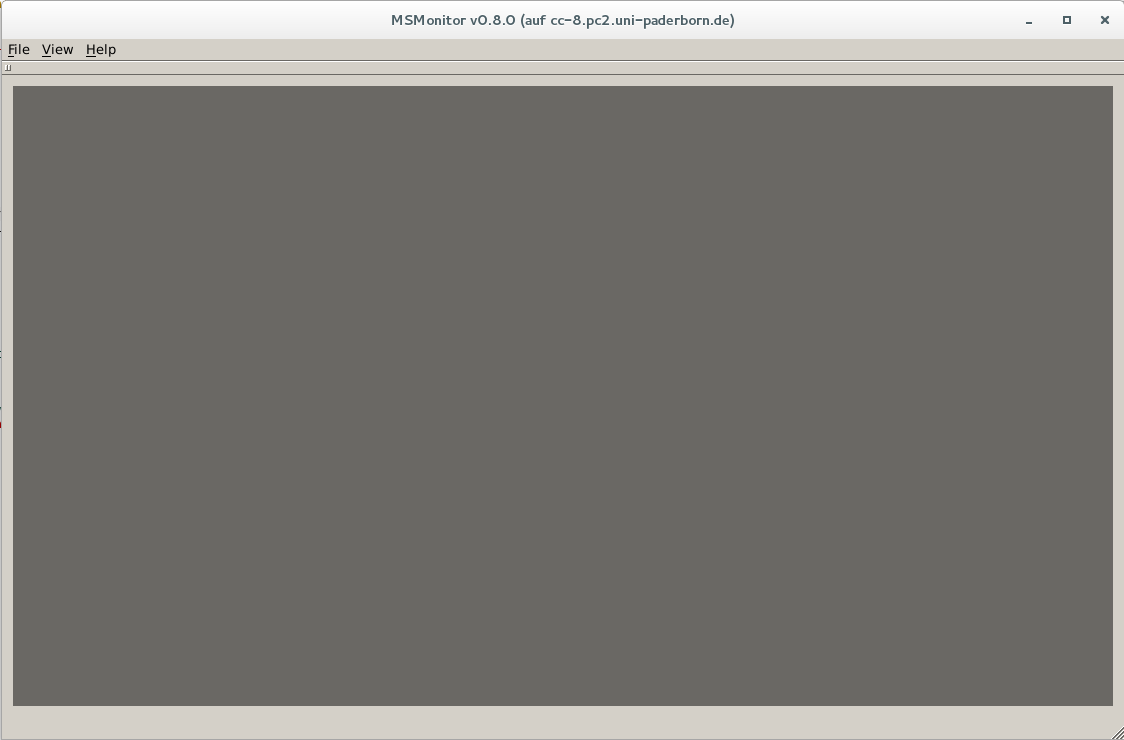
\includegraphics[width=0.9\textwidth]{msm_blank.png} 
		\caption{Starting user interface of MSMonitor}
		\label{fig:msm_blank}
	\end{center}
\end{figure}
The settings window and all the plots can be opened from the menu bar or via keyboard shortcuts. They appear on the mdi area, where users can move them around.\newline
The settings window contains all controls to connect to the server, set up the GUI refresh rate and data frequency. This can be seen in Figure \ref{fig:msm_settings}. The data frequency sets the interval of time, in which new data is being requested from the server. The Save Data spinbox sets the amount of values to be drawn. Setting this to 1 would only draw a point. If "Save Data" is set to 100 and the amount of available data exceeds 100, then the oldest data will be erased until the amount of available data is less or equal 100.\newline The GUI refresh rate sets the interval of time, in which the graphs are being redrawn, no matter if new data is already available or not.\newline Tooltips are available for each setting, in order to receive further information.\newline In order to connect to the server, its IP address and port need to be given. In case a firewall is set up on the heterogeneous node, a direct connection is prohibited. In this case a ssh tunnel can be used as a workaround.\newline
After compiling the client run the client script to set up the tunnel:
\begin{lstlisting}[caption={install the client}, label=lst:msg4]
git clone https://github.com/akiml/ampehre.git
cd ampehre
make client
./msmonitor_client.sh "<IP_ADDRESS>" <PORT>
\end{lstlisting}
The first argument is the IP address of the server and the second argument is the port number.\newline
The settings can be exported to a configuration file, which can be loaded on the next session.
\begin{figure}[t!]
	\begin{center}
		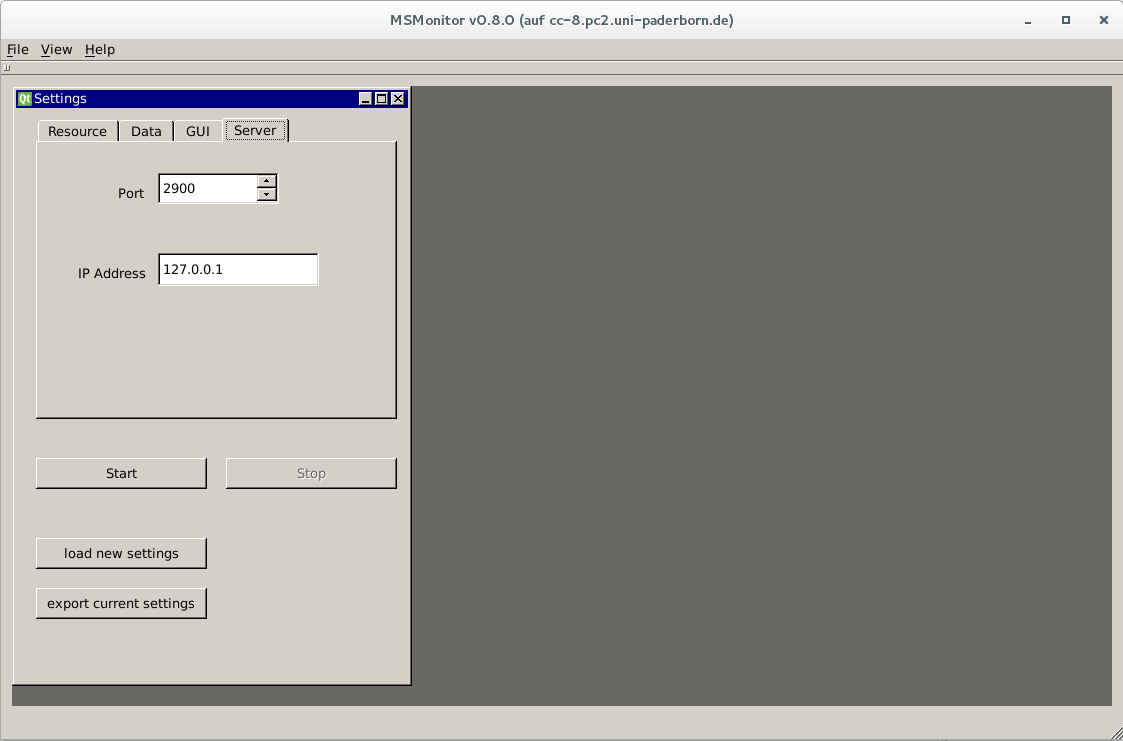
\includegraphics[width=0.9\textwidth]{msm_settings.png} 
		\caption{User interface after enabling the settings window}
		\label{fig:msm_settings}
	\end{center}
\end{figure}
After connecting to the server, the plots will be drawn.\newline 
Each consists of two tabs. The first tab (plot) contains the coordinate system itself, a legend, a spin box to choose the thickness of the curves , a screenshot button to export the current graph to png and a csv export button to export the values into a highly manageable comma separated format. This can be seen in Figure \ref{fig:msm_graph}.
\begin{figure}[t!]
	\begin{center}
		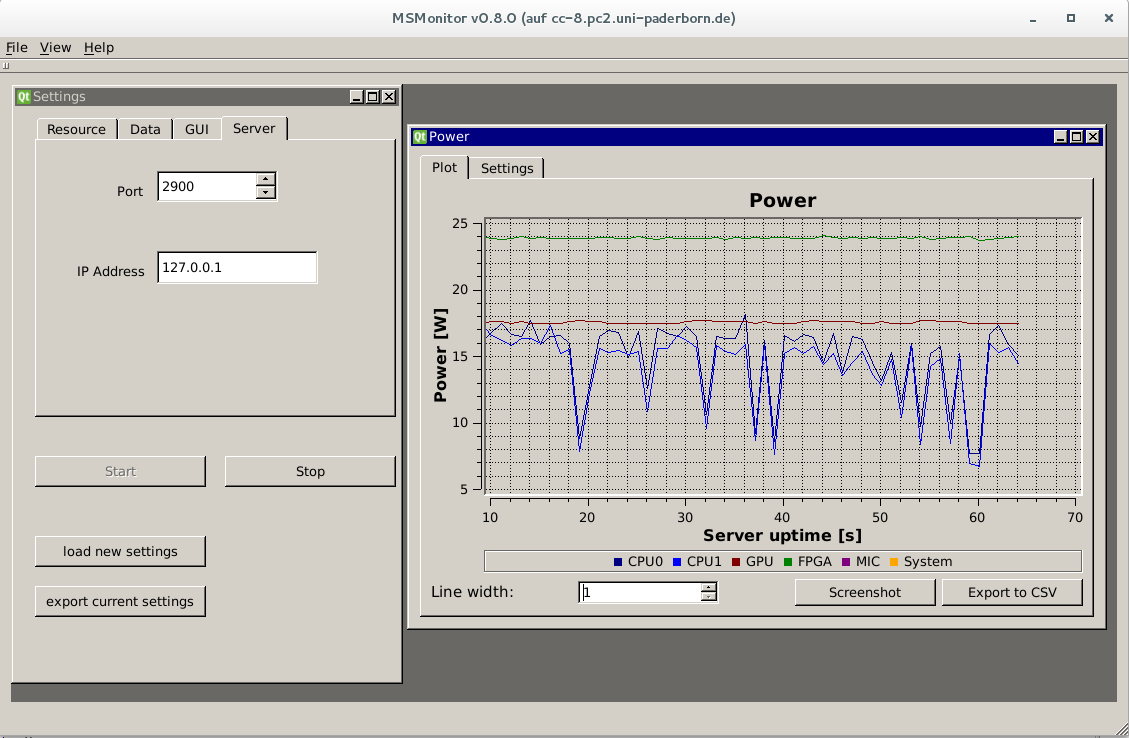
\includegraphics[width=0.9\textwidth]{msm_graph.png} 
		\caption{Active graph in msmonitor (right)}
		\label{fig:msm_graph}
	\end{center}
\end{figure}
The second tab (settings), shown in Figure \ref{fig:msm_secondTab}, gives the option to enable or disable currently drawn graphs by simply clicking on the corresponding labels. Recorded global minimum and maximum values are listed next to the labels and can also be shown inside the graph.\newline
If the curves have high fluctuation, median and mean filter can be applied over a user-specified interval, in order to clarify tendencies. Please note, if the chosen interval is higher than the actual amount of values, nothing will be plotted until the amount of recorded data exceeds the chosen interval.
\begin{figure}[t!]
	\begin{center}
		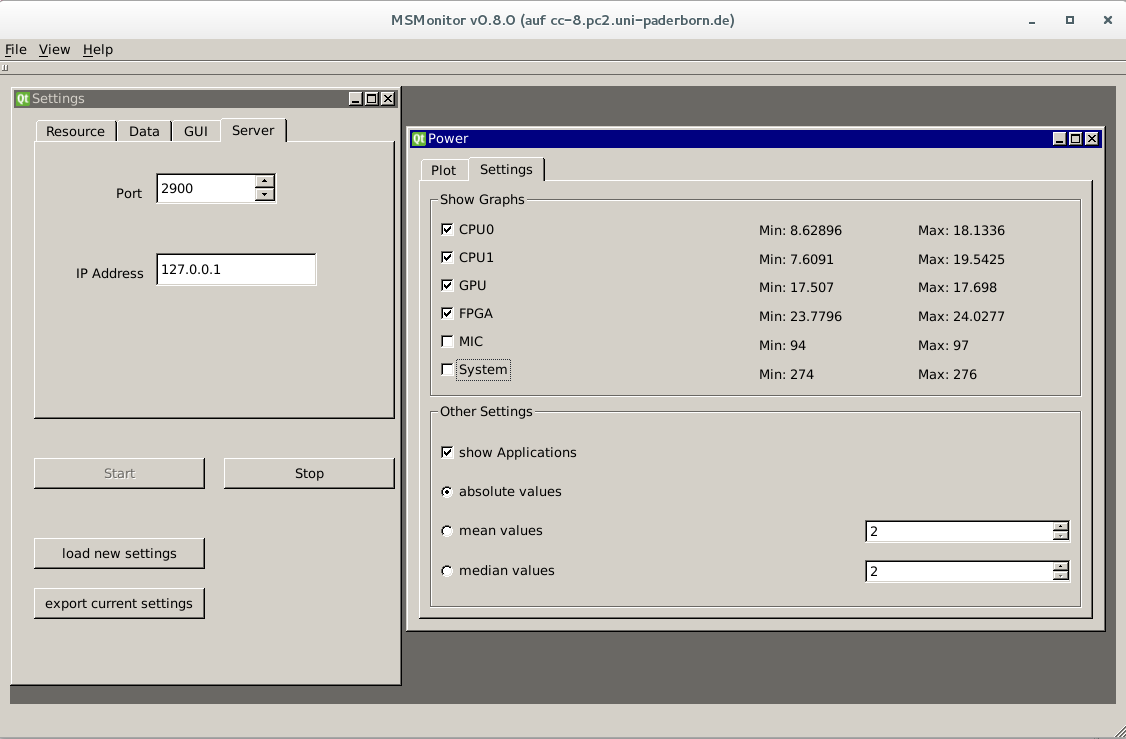
\includegraphics[width=0.9\textwidth]{msm_secondTab.png} 
		\caption{Second tab of a plot (right)}
		\label{fig:msm_secondTab}
	\end{center}
\end{figure}
Besides the option of drawing graphs, start and termination of specific programs can be symbolized on the graphs, by sending UNIX signals SIGUSR1 and SIGUSR2 to the server. If SIGUSR1 is signaled to the server prior to starting, it informs the clients about a newly started application. Sending SIGUSR2, informs all registered clients about the termination of an application. The unique process ID ensures that the user can identify the lifetime of an application.\newline
Besides the mentioned graphs and curves there are also other forms of visualization available. The heatmaps give a feedback using a defined color-scale. For example high temperature will be presented in red and low temperature in blue.\newline
The system overview gives a summary about current processes on the heterogeneous node and gives an overview over most of the currently measured data.  



